\documentclass[a4paper]{article}
\usepackage[margin=1in]{geometry}

\usepackage{minted}

\usepackage{hyperref}

\usepackage{float}
\restylefloat{table}
\usepackage{booktabs}

\usepackage{indentfirst}
\usepackage{url}
\usepackage{csquotes}

\usepackage{algorithm}
\usepackage[noend]{algpseudocode}

\usepackage{graphicx}
\graphicspath{ {./images/} }

\usepackage{enumitem}
\newlist{steps}{enumerate}{1}
\setlist[steps, 1]{label = Step \arabic*:}

\title{T2 - Numerical optimization using Genetic Algorithms}
\author{Oloieri Alexandru}
\date{November 25, 2019}


\begin{document}
	
	\maketitle
	
	\begin{abstract}
		\centering
		This paper analyzes the behaviour and performance of Genetic Algorithms when dealing with a complex problem: finding the global minima/maxima of a mathematical benchmark function, and compares the obtained results with the results of a well known trajectory-based method: Hill Climbing Best Improvement.
	\end{abstract}
	
	\section{Introduction}
	
	In computer science, there are some problems which require a lot of resources (time, memory) in order to be solved (usually these are called hard problems), and, unfortunately, classical algorithms are too weak for solving them. One way to solve this kind of problems is using metaheuristics, because even if they don't produce an optimal result on each run, the results they produce are usable and most of the times their running time is low compared to other algorithms that would find the optimal result, but realistically speaking, they would never end for large instances of the problem.
	
	A well known hard problem is finding the global minimum/maximum of a mathematical benchmark function which is defined on an interval, because a computer cannot run an algorithm that evaluates the function in each point from the function domain, and then chooses the best one (because there are an infinity of points). This paper analyzes how good are Genetic Algorithms behaving in practice, when dealing with this problem, more exactly, when trying to find the global minimum of some functions with more than one dimensions (functions which have an argument of type $x = (x_1,x_2,...,x_n)$). 
	
	\section{Genetic Algorithm Description}
	
	In computer science and operations research, a genetic algorithm (GA) is a metaheuristic inspired by the process of natural selection. \cite{GA}
	Genetic algorithms are a population-based approach, as they maintain and improve multiple candidate solutions, often using population characteristics to guide the search and relying on bio-inspired operators such as mutation, crossover and selection. \cite{GA} \cite{Metaheuristics} 
	In this experiment the size of the populations at each iteration will be equal to $populationSize = 100$. 
	
	\subsection{Representation of the solutions}
	
	The solutions will be represented as binary arrays. Let's say we want to represent every real number with $d$ digits for precision. Then we will divide the function domain $\left[leftMargin, rightMargin\right]$ in $Cnt=(rightMargin-leftMargin)*10^d$ equal intervals. For a dimension, to represent $Cnt$ different values we need $len=\lceil log2(Cnt)\rceil$ bits, so for $N$ dimensions, for each chromosome, we will need $len \cdot N$ bits. In this experiment the precision will be $d = 5$.
	
	\subsection{Decodification of the solutions}
	
	We will have to decode the solutions to be able to evaluate them. If we represented real numbers in the manner described at 2.1, then for a function with $N$ dimensions, the following domain: $\left[leftMargin, rightMargin\right]$, and $binary_i$ being the binary representation of the $i^{th}$ dimension, the real value for each dimension will be:
	
	$$ realValue_i = leftMargin+decimal(binary_i)/(2^{len}-1) \cdot (rightMargin - leftMargin) $$
	
	\subsection{Crossover}
	
	Crossover (also called recombination) is a genetic operator used to combine the genetic information of two parents to generate new offspring. \cite{Crossover} During an iteration each chromosome will have a crossover probability $p_i$, and those who have $p_i < P_{c}$, where $P_{c}$ is the crossover probability constant, will take part in crossover.
	
	\subsection{Mutation}
	
	Mutation is a genetic operator used to maintain genetic diversity from one generation of a population of genetic algorithm chromosomes to the next. It is analogous to biological mutation. Mutation alters one or more gene values in a chromosome from its initial state. The purpose of mutation in GAs is preserving and introducing diversity. Mutation should allow the algorithm to avoid local minima by preventing the population of chromosomes from becoming too similar to each other, thus slowing or even stopping evolution.\cite{Mutation} This will be implemented in the following way: each bit from the cromosome will have its value changed with a probability equal to $P_{m}$.
	
	\subsection{Selection}
	
	During each successive generation, a portion of the existing population is selected to breed a new generation. Individual solutions are selected through a fitness-based process, where fitter solutions (as measured by a fitness function) are typically more likely to be selected.\cite{GA} Since all the benchmark functions used in the experiemnt evaluate only to positive values, the fitness function that will be used is:
	$$ fitness_{i} = 1 / (f(chromosome_i) + 0.01) $$
	
	\subsection{Elitism}
	
	A practical variant of the general process of constructing a new population is to allow the best organism(s) from the current generation to carry over to the next, unaltered. This strategy is known as elitist selection and guarantees that the solution quality obtained by the GA will not decrease from one generation to the next. \cite{GA} This will be achieved by copying the best $k_{e}$ candidates from the current generation to the next one (during the selection stage).
	
	\subsection{Final Algorithm}
	
	\begin{algorithm}
		\caption{Genetic Algorithm Scheme}
		\begin{algorithmic}[1]
			\State $population \gets randPopulation()$;
			\For {$i \gets 2; i \leq generationsCount; ++i$}
			\State $mutation()$;
			\State $crossOver()$;
			\State $population \gets selection(population)$;
			\EndFor
			\State $return$ $best(population)$;
		\end{algorithmic}
	\end{algorithm}
	
	\section{Functions}
	
	Rastrigin's function:
	$$ f(x) = A \cdot n + \sum_{i=1}^n \left[ x_i^2 - A \cdot cos(2 \pi x_i) \right],
	A = 10, x_i \in \left[ -5.12, 5.12 \right]$$
	
	Schwefel's function:
	$$ f(x) = 418.9829\cdot n - \sum_{i=1}^n \left[ x_i \cdot sin(\sqrt{|x_i|}) \right], x_i \in \left[ -500.0, 500.0\right]$$
	
	Griewank's function:
	$$ f(x) = 1 + \sum_{i=1}^n \left[ x_i^2/4000 \right] - \prod_{i=1}^n \left[cos(x_i/\sqrt{i})\right], x_i \in \left[-600.0, 600.0 \right]$$
	
	Zakharov's function:
	$$ f(x) = \sum_{i=1}^{n} x_i^2 + (\sum_{i=1}^n 0.5 \cdot i \cdot x_i)^2 + (\sum_{i=1}^n 0.5 \cdot i \cdot x_i)^4, x_i \in \left[ -5.0, 10.0 \right]$$
	\\
	
	%Rosenbrock's function:
	%$$ f(x) = \sum_{i=1}^{n-1} \left[ 100 \cdot (x_i^2 - x_{i+1})^2 + (1 - x_i)^2 \right],
	%x_i \in \left[ -5.0, 10.0\right]$$
	
	%De Jong's function:
	%$$ f(x) = \sum_{i=1}^{n} x_i^2, x_i \in \left[ -5.12, 5.12 \right]$$
	
	For the experiment to have varied and relevant results, appropriate functions have to be chosen (with different types of plots and different properties). For that, in this experiment three non-convex and multimodal functions, with a lot of local minimas (Rastrigin's function, Schwefel's functions and Griewank's function) and one unimodal and convex function, with no local minimum except the global one (Zakharov's function) will we used.
	
	\section{Experiment}
	
	\subsection{Suggested parameters analysis}
	
	The suggested parameters for running the genetic algorithms are: 
	
	\begin{itemize}
		\item $populationSize = 100$
		\item $generationsCount = 1000$
		\item $crossOverProbability (P_{c}) = 0.3$
		\item $mutationProbability (P_{m}) = 0.01$
	\end{itemize}
	
	\begin{figure}[!h]
		\centering
		\begin{tabular}{|| c | c | c | c | c | c | c | c ||}
			\hline
			dim & runs & generationsCount & best & worst & mean & stDev & time(s) \\ \hline \hline
			5 & 15 & 1000 & 6.18 & 20.05 & 14.89 & 3.56 & 4.8 \\ \hline
		\end{tabular}
		\caption{Rastrigin's function results with suggested parameters}
	\end{figure}
	
	The results for the Rastrigin's function with 5 dimensions are pretty bad, as even the Naive Hill Climbing provides better results (even though that strategy gets stuck in a local minima). In my opinion this is due to the values provided by the fitness function, because they are very close one to each other, and the best chromosomes don't have significant better chance to be selected (the selection pressure is low, and this is a disadvantage for fit candidates). This together with the high rate of mutation makes the algorithm to sometimes "lose" the best candidades. But the benefit of metaheuristics is that we can experiment with several values for parameters, and then choose the ones that fit the best our needs, so an idea is to modify some of the parameters in trying to get the best possible results.
	
	\subsubsection{Generations Count}
	
	After increasing the generations count to 7500, the running time increased, but the results were better, because even if the mutation affected the best chromosomes, there were more iterations when the GA could improve the results.
	
	\begin{figure}[!h]
		\centering
		\begin{tabular}{|| c | c | c | c | c | c | c | c ||}
			\hline
			dim & runs & generationsCount & best & worst & mean & stDev & time(s) \\ \hline \hline
			5 & 15 & 1000 & 5.05 & 12.03 & 9.19 & 2.23 & 73.664 \\ \hline
		\end{tabular}
		\caption{Rastrigin's function results with increased generations count}
	\end{figure}
	
	\subsubsection{Mutation probability and Elitism}
	
	To further optimize the algorithm, the mutationProbability was lowered to $P_{m} = 0.001$, and also the strategy described at \textbf{2.6} (Elitism, $k_{e} = 6$) was integrated in the program, and this led to very close to optimal results.
	
	\begin{figure}[!h]
		\centering
		\begin{tabular}{|| c | c | c | c | c | c | c | c ||}
			\hline
			dim & runs & generationsCount & best & worst & mean & stDev & time(s) \\ \hline \hline
			5 & 15 & 1000 & 0.00 & 4.46 & 1.06 & 1.59 & 44.13 \\ \hline
		\end{tabular}
		\caption{Rastrigin's function results with some optimizations}
	\end{figure}
	
	\subsection{Parameters used in the experiment}
	
	As the goal of using Genetic Algorithms is to get best possible results, some of the suggested parameters will be modified to increase the selection pressure and to ensure that, for most of the times, the quality of the best candidate will not decrease between generations.
	
	\begin{itemize}
		\item $populationSize = 100$
		\item $ generationsCount = 10.000 $ for 10 and 30 dimensions, $generationsCount = 7.500$ for 5 dimensions
		\item $ P_{m} = 0.001 $
		\item $crossOverProbability (P_{c}) = 0.3$
		\item $ k_{e} = 6 $ (best 6 chromosomes will be copied from the current generation to the next one)
	\end{itemize}
	
	For each function and for each number of dimensions, the Genetic Algorithm described at \textbf{Section 2} will be run 30 times using the above parameters.
	
	%\clearpage
	
	\section{Results}
	
	\begin{figure}[!h]
		\centering
		\begin{tabular}{|| c | c | c | c | c | c | c ||}
			\hline
			dim & generationsCount & best & worst & mean & stDev & time(s) \\ \hline \hline
			5 & 7500 & 0.00 & 5.62 & 1.53 & 1.68 & 76.094 \\ \hline
			10 & 10000 & 0.00 & 8.63 & 3.86 & 2.84 & 197.45 \\ \hline
			30 & 10000 & 11.16 & 42.19 & 23.6 & 7.41 & 569.203 \\ \hline
		\end{tabular}
		\caption{Rastrigin's function results}
	\end{figure}
	
	\begin{figure}[h]
		\centering
		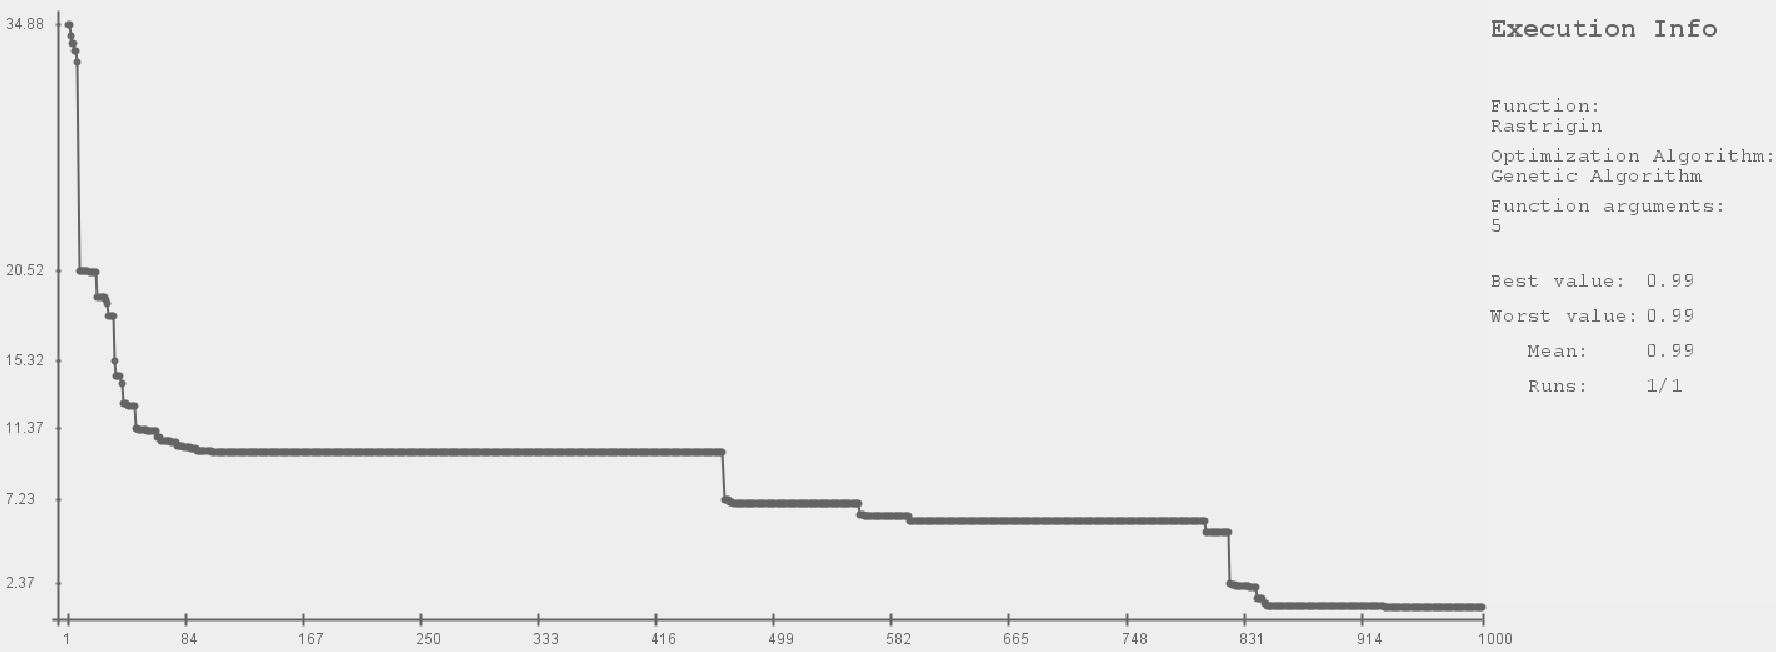
\includegraphics[width=16cm]{rastrigin_5_1000.JPG}
		\caption{Rastrigin's function 5 dimensions, 1000 generations}
	\end{figure}
	
	\begin{figure}[!h]
		\centering
		\begin{tabular}{|| c | c | c | c | c | c | c ||}
			\hline
			dim & generationsCount & best & worst & mean & stDev & time(s) \\ \hline \hline
			5 & 7500 & 0.103 & 0.51 & 0.27 & 0.12 & 93.81 \\ \hline
			10 & 10000 & 0.106 & 34.73 & 2.76 & 8.53 & 248.14 \\ \hline
			30 & 10000 & 36.0 & 727.45 & 246.18 & 144.03 & 723.13 \\ \hline
		\end{tabular}
		\caption{Schwefel's function results}
	\end{figure}
	
	\begin{figure}[h]
		\centering
		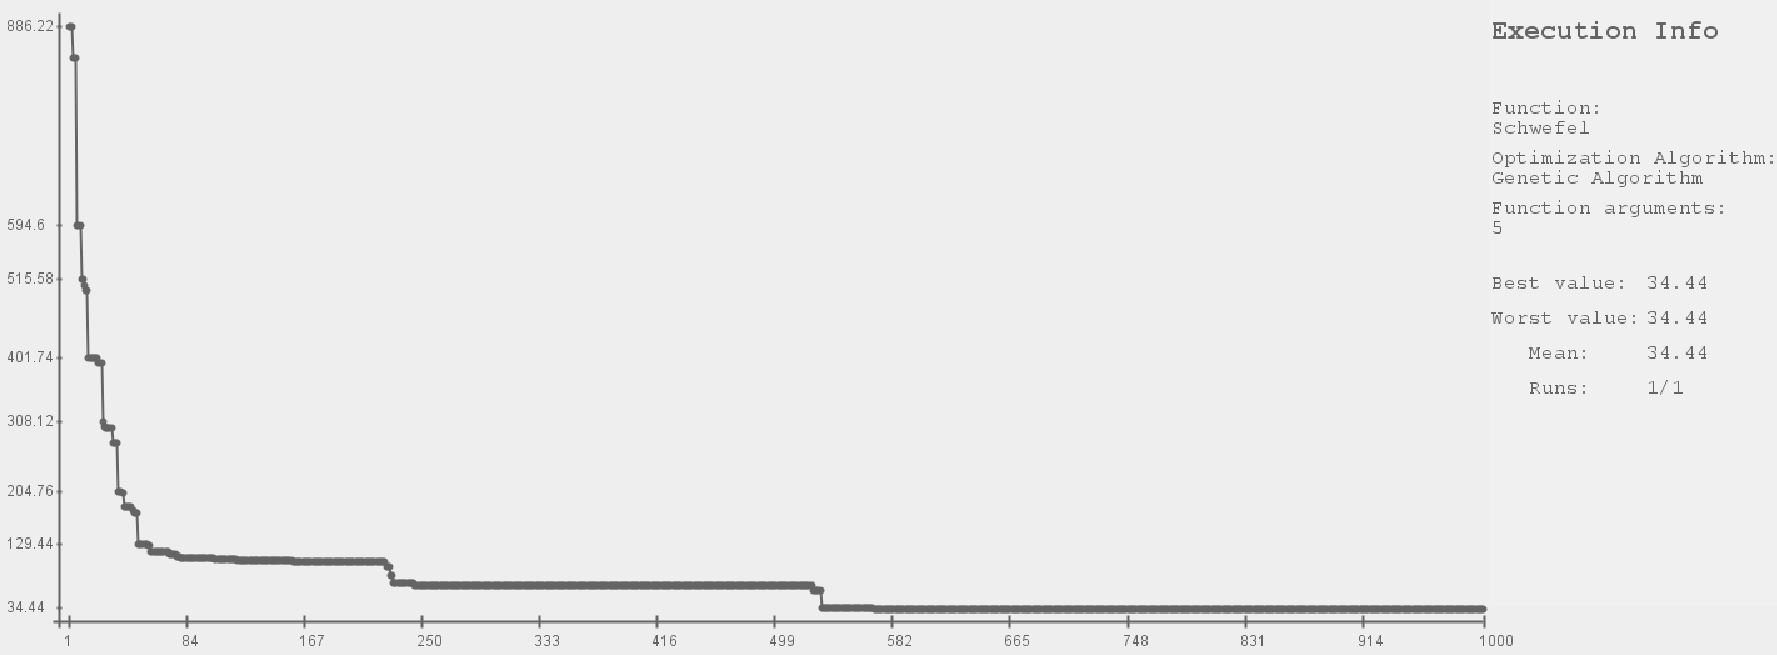
\includegraphics[width=16cm]{schwefel_5_1000.JPG}
		\caption{Schwefel's function 5 dimensions, 1000 generations}
	\end{figure}
	
	\begin{figure}[!h]
		\centering
		\begin{tabular}{|| c | c | c | c | c | c | c ||}
			\hline
			dim & generationsCount & best & worst & mean & stDev & time(s) \\ \hline \hline
			5 & 7500 & 0.007 & 0.16 & 0.04 & 0.034 & 80.95 \\ \hline
			10 & 10000 & 0.00 & 0.19 & 0.07 & 0.04 & 212.63 \\ \hline
			30 & 10000 & 0.10 & 0.25 & 0.08 & 0.05 & 622.93 \\ \hline
		\end{tabular}
		\caption{Griewank's function results}
	\end{figure}
	
	\begin{figure}[!h]
		\centering
		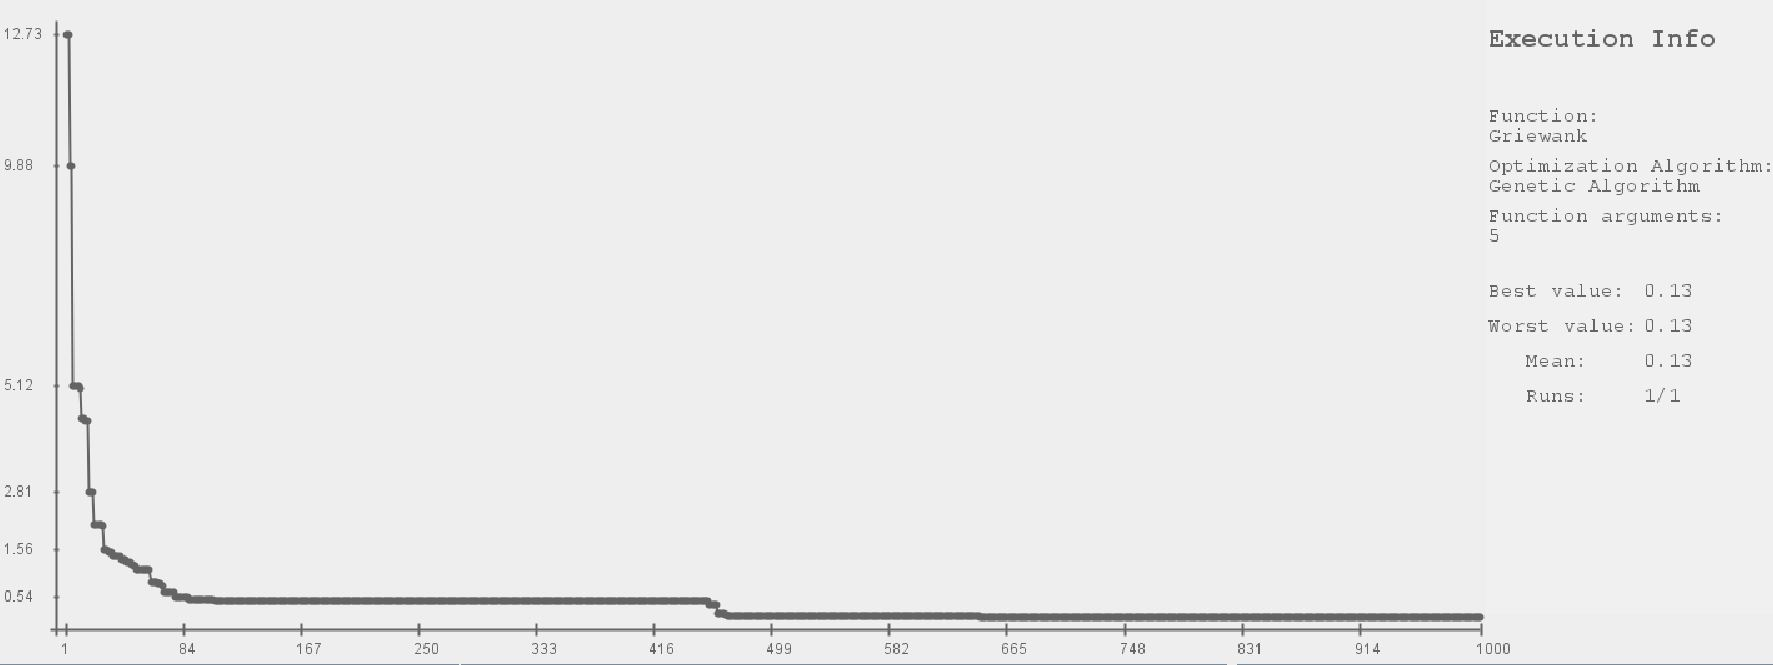
\includegraphics[width=16cm]{griewank_5_1000.JPG}
		\caption{Griewank's function 5 dimensions, 1000 generations}
	\end{figure}
	
	\begin{figure}[!h]
		\centering
		\begin{tabular}{|| c | c | c | c | c | c | c ||}
			\hline
			dim & generationsCount & best & worst & mean & stDev & time(s) \\ \hline \hline
			5 & 7500 & 0.03 & 11.79 & 3.86 & 3.67 & 63.91 \\ \hline
			10 & 10000 & 1.13 & 26.43 & 12.59 & 6.39 & 155.074 \\ \hline
			30 & 10000 & 38.56 & 71.15 & 57.12 & 8.84 & 464.87 \\ \hline
		\end{tabular}
		\caption{Zakharov's function results}
	\end{figure}
	
	\begin{figure}[!h]
		\centering
		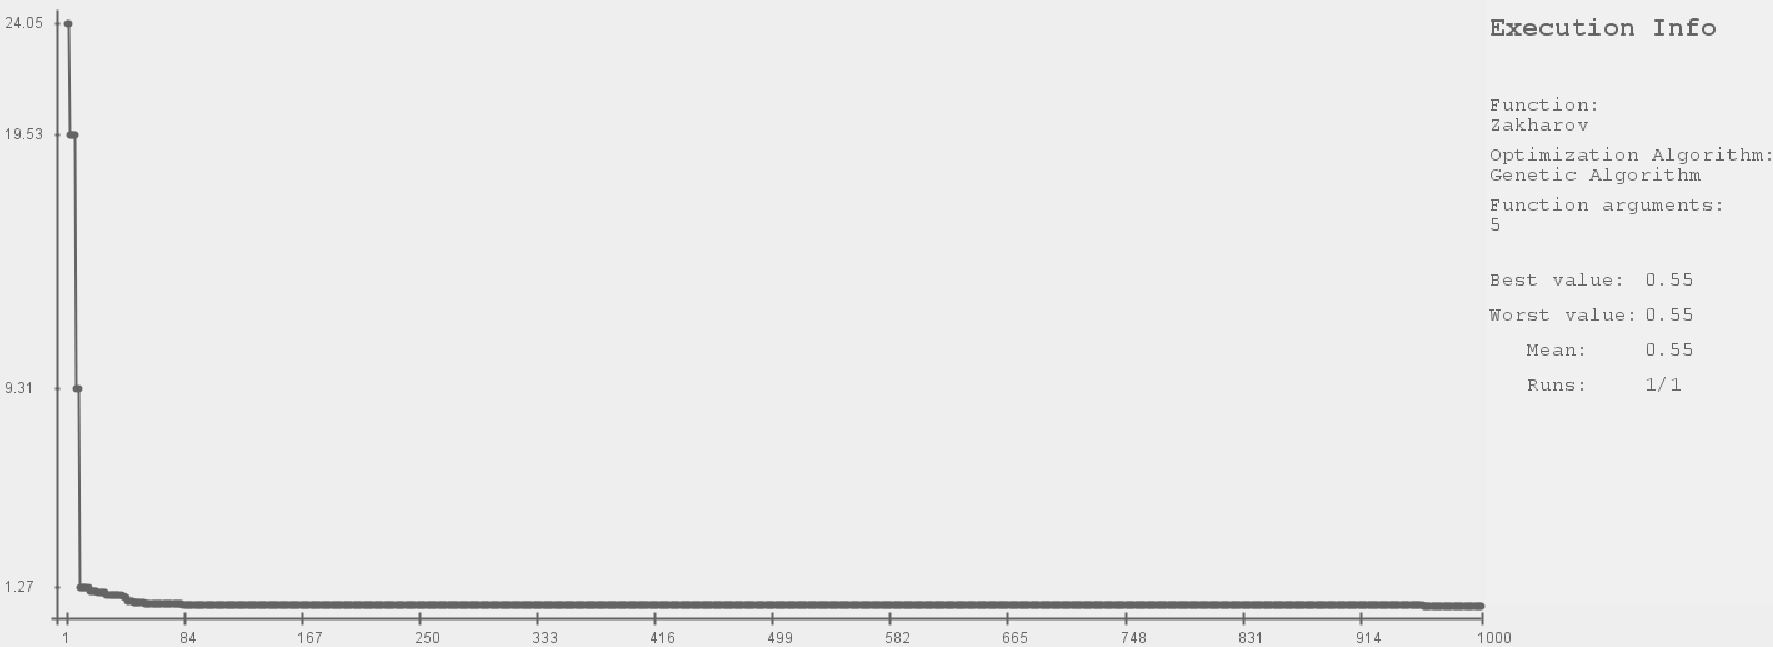
\includegraphics[width=16cm]{zakharov_5_1000.JPG}
		\caption{Zakharov's function 5 dimensions, 1000 generations}
	\end{figure}
	
	\subsection{Interpretation}
	
	\subsubsection{Rastrigin's, Schwefel's and Griewank's functions}
	
	The obtained results for these functions are very close to the global optimum, and this is mainly due to the optimizations added to the standard Genetic Algorithm (Elitism and a smaller value for mutation probability), which guaranteed that the best solution quality will not decrease from one generation to another.
	
	An interesting thing to observe is that for Griewank's function, the results are very close to global minimum for all the dimensions (whereas for most functions the global minima increases as we increase the number of dimensions). That's because the way we chose the fitness function ($1 / f(x)$) really benefits the functions which have large values in function codomain, and the function domain is $\left[ -600.0, 600.0 \right]$, so $f(x)$ will be pretty large, so during the selection phase best candidates will have a very high chance to be selected. This together with the fact that elitism was integrated in the algorithm almost guarantees that we will get good results (results close to the optimum).
	
	As $generationsCount$ is fixed (7.500 for 5 dimensions and 10.000 for 10 and 30 dimensions), the running time of the algorithms are very similar, the small differences are only caused by the complexity of the operations needed for evaluating a function. (for example, computing the square root of some real numbers, the sine of a value etc.)
	
	\subsubsection{Zakharov's function}
	
	The way the GA was implemented doesn't guarantee that for convex functions it will find the global minima on each run (unlike the Hill Climbing or Simulated Annealing strategies). This is because the mutations may modify some bits of the best candidates, so they cannot converge to the global minima. Since the values of the function evaluations are small and close to each other (so there is a small selection pressure), during selection we may miss choosing the best chromosomes. The running times are a little bit smaller than the running time of the other functions because this function only contains basic mathematical operations: addition and multiplication (so we need less computational effort). Something very interesting is that the best candidate improved a lot during the first 50/60 iterations, and then there was barely any improvement, and I think that's mainly because the genetic operators (mutation and crossover) affected the best candidates, so no chromosome could converge to the global minima.
	
	\subsubsection{Comparison with Hill Climbing Best Improvement}
		
	\begin{itemize}
		\item Multimodal functions
		
		\begin{figure}[!h]
			\centering
			\begin{tabular}{||c |  c | c | c | c | c | c | c ||}
				\hline
				algorithm & dim & generationsCount & best & worst & mean & stDev & time(s) \\ \hline \hline
				Genetic Algorithm & 30 & 10000 & 11.16 & 42.19 & 23.6 & 7.41 & 569.203 \\ \hline
				HC Best Improvement & 30 & - & 26.26 & 40.83 & 34.04 & 3.92 & 399.78 \\ \hline
			\end{tabular}
			\caption{Rastrigin's function results comparison}
		\end{figure}
	
		\begin{figure}[!h]
		\centering
		\begin{tabular}{||c |  c | c | c | c | c | c | c ||}
			\hline
			algorithm & dim & generationsCount & best & worst & mean & stDev & time(s) \\ \hline \hline
			Genetic Algorithm & 30 & 10000 & 36.0 & 727.45 & 246.18 & 144.03 & 723.13 \\ \hline
			HC Best Improvement & 30 & - & 723.32 & 1817.14 & 1498.29 & 216.901 & 974.66 \\ \hline
		\end{tabular}
		\caption{Schwefel’s function results comparison}
		\end{figure}
		
		For non-convex and unimodal functions the Genetic Algorithm found way better results than the Hill Climbing one, because most of the times, due to the greedy strategy it uses, the Hill Climbing algorithm gets stuck in local minimas, whereas the Genetic Algorithm not only maintains more than one solution, but also uses the genetic operators described at \textbf{2.3} and \textbf{2.4} which will cause a better exploration and exploitation of the function domain. The running time of the Genetic Algorithm is almost constant for a fixed $populationsCount$, in contrast to the running time of the Hill Climbing strategy, which will vary based on the function graph and the quality of the neighbors (the number of times we find a better candidate during iterations may be very large).
	
		\item Unimodal functions
		
		\begin{figure}[!h]
			\centering
			\begin{tabular}{||c |  c | c | c | c | c | c | c ||}
				\hline
				algorithm & dim & generationsCount & best & worst & mean & stDev & time(s) \\ \hline \hline
				Genetic Algorithm & 20 & 10000 & 28.36 & 65.14 & 39.78 & 9.28 & 164.03 \\ \hline
				HC & 20 & - & 0.00 & 0.00 & 0.0 & 0.0 & 52.58 \\ \hline
			\end{tabular}
			\caption{Zakharov’s function results comparison}
		\end{figure}
	
		The strategy of the Hill Climbing algorithms is perfect for this kind of functions because it doesn't matter what is the starting point, it will always converge to the global minima. This is not the case for Genetic Algorithms, and this can be observed from the results: because the number of generations was 10000 it had a higher running time, and the results were worse.
	
	\end{itemize}
	
	\section{Conclusions}
	
	Even though they are complex, when used with wrong parameters, Genetic Algorithms can have worse results than simpler optimization strategies, as observed in section \textbf{4.1}, so with a little bit of analysis suitable/optimal parameters can be chosen, and when this happens, the results are better than the ones provided by other strategies like Hill Climbing or Simulated Annealing, with comparable running times that can also be adjusted when increasing or decreasing the value of $populationsCount$. So this metaheuristic is a good option for the cases when we need both accuracy (get the best possible results) and efficiency (the execution time to be as low as possible), but it must be taken into account that it doesn't benefit specific types of functions (which happens for Hill Climbing algorithms and unimodal functions), so there are cases when the results are worse, and other strategies should be used. 
	
	Consequently, Genetic Algorithms are powerfull algorithms, with relative low running time, that when used correctly can generate better results than other metaheuristics.
	
	\begin{thebibliography}{9}
		
		\bibitem{GA}
		More about GAs in computer science:
		\url{https://en.wikipedia.org/wiki/Genetic_algorithm}
		
		\bibitem{Metaheuristics}
		More about metaheuristics in computer science:
		\url{https://en.wikipedia.org/wiki/Metaheuristic}
		
		\bibitem{Mutation}
		More about mutation in GAs:
		\url{https://en.wikipedia.org/wiki/Mutation_(genetic_algorithm)}
		
		\bibitem{Crossover}
		Crossover in GAs:
		\url{https://en.wikipedia.org/wiki/Crossover_(genetic_algorithm)}
		
		\bibitem{Functions}
		Information about functions used in this experiment:
		\url{https://www.sfu.ca/~ssurjano/optimization.html}
		
		\bibitem{Implementation details}
		More details about the implementation of genetic algorithms:
		\url{https://profs.info.uaic.ro/~pmihaela/GA/laborator3.html}
		
		\bibitem{Numerical optimization plaftorm}
		The github repository of the application used in this experiment:
		\url{https://github.com/OloieriAlexandru/Numerical-Optimization-Platform/tree/T2}
		
	\end{thebibliography}
	
\end{document}

